%==================================================================================================================================%
%==================================================== 第三章 曲面上的 SCFT 模型 ====================================================%
%==================================================================================================================================%

\chapter{Lévy-Feller对流-扩散方程的数值解法} \label{Chap:Surface_SCFT}

1905年,Einstein根据布朗运动现象第一次提出扩散方程,而分数阶对流—扩散方程直接来源于这个结果的推广,并且断言其可以用来描述反常扩散过程。分数阶对流—扩散方程的解为一个Stable分布函数——方差无穷大的独立同分布的随机变量序列的极限分布函数。本章着重探讨的是Lévy-Feller对流-扩散方程。

\section{Lévy-Feller对流-扩散方程的有关知识}
Lévy-Feller对流-扩散方程表达的是满足某种稳定分布反常扩散的非对称空间分数阶对流-扩散方程\cite{lqx2007}。

\subsection{Lévy-Feller对流-扩散方程的表达式}
首先引入Lévy-Feller对流—扩散微分方程:
\begin{equation} 
\frac{\partial u(x, t)}{\partial t}=a D_{\theta}^{\alpha} u(x, t)-b \frac{\partial u(x, t)}{\partial x}
\end{equation}
其中a为正常数,b为常数,算子$D^{\alpha}_{\theta}$表示阶数为$\alpha$、倾斜度为$\theta$的Riesz-Feller分数阶导数。Riemann-Liouville分数阶导数以其Fourier变换形式给出:
\begin{equation} 
\widehat{D}_{\theta}^{\alpha}=-|\kappa|^{\alpha} e^{i(\operatorname{sign} \kappa) \theta \pi / 2}
\end{equation}

由文献\cite{lqx2007}中的内容可知:
$$D_{\theta}^{\alpha}=-\left[c_{+}(\alpha, \theta) \frac{d^{\alpha}}{d x^{\alpha}}+c_{-}(\alpha, \theta) \frac{d^{\alpha}}{d(-x)^{\alpha}}\right]$$
其中$\frac{d^{\alpha}}{dx^{\alpha}}$和$\frac{d^{\alpha}}{d(-x)^{\alpha}}$分别为左侧和右侧Riemann-Liouville分数阶导数算子。系数c+、c-如下:
\begin{equation*}
		\left\{
	\begin{aligned}
		& c_{+} = c_{+}(\alpha,\theta) := \frac{sin((\alpha-\theta)\pi/2)}{sin(\alpha\pi)}
	\\	& c_{-} = c_{-}(\alpha,\theta) := \frac{sin((\alpha+\theta)\pi/2)}{sin(\alpha\pi)}
	\end{aligned}
	\right.	
\end{equation*}
其中参数$\alpha$、$\theta$满足:
\begin{equation*}
	0 < \alpha \leq 2(\alpha \neq 1);\quad |\theta| \leq \left\{
	\begin{aligned}
		& \alpha, 0 < \alpha <1
	\\  & 2-\alpha, 1 < \alpha \leq 2.
	\end{aligned}
	\right.
\end{equation*}
在此给出参数$c_{+}、c_{-}$的性质:
\begin{equation*}
c_{\pm}\left\{
\begin{aligned}
& \geq 0, 0 < \alpha <1
\\  & \leq 0, 1 < \alpha \leq 2.
\end{aligned}
\right.	
\end{equation*}

\begin{lemma}
	初边值条件如下:
	\begin{equation*}
		\left\{
		\begin{aligned}
			& u(x, 0)=\varphi(x), \quad (x \in \mathbb{R}) 
			\\	& u( \pm \infty, t)=0, \quad (t>0)
		\end{aligned}
		\right.
	\end{equation*}	
	的Lévy-Feller对流-扩散方程的解析解为
	\begin{equation*}
		\begin{aligned}
			u(x, t) =\frac{1}{2 \pi} \int_{-\infty}^{+\infty+\infty} e^{-i \kappa \xi} e^{t\left(-a|\kappa|^{\alpha} e^{i(s i g n \kappa) \theta \pi / 2}+i b \kappa\right)} \varphi(x-\xi) d \kappa d \xi
		\end{aligned}
	\end{equation*}
\end{lemma}

详细证明请参考文献\cite{lqx2007}。



\subsection{有限区间内的初边值问题的数值解法}
给出初边值问题如下;
\begin{equation} 
\begin{array}{ll}{\frac{\partial u(x, t)}{\partial t}=a D_{\theta}^{\alpha} u(x, t)-b \frac{\partial u(x, t)}{\partial x},} & {0<x<R, \quad 0<t<T} \\ {u(x, 0)=\varphi(x),} & {0 \leq x \leq R} \\ {u(0, t)=u(R, t)=0,} & {0 \leq t \leq T}\end{array}
\end{equation}

先进行网格剖分,将空间区间[0,L]作M等分,时间区间[0,T]作N等分。其中$h$和$\tau$分别表示空间步长和时间步长,M和N为给定正整数。

利用空间网格点
$$x_{j}=jh,h>0,j=0,\pm1,\pm2,...$$
和时间间隔
$$t_{n}=n\tau,\tau>0,n=0,1,2,...$$
离散空间和时间变量。引入$y_{j}(t_{n})$:
$$y_{j}\left(t_{n}\right)=\int_{x_{j}-h / 2}^{x_{j}+h / 2} u\left(x, t_{n}\right) d x \approx h u\left(x_{j}, t_{n}\right)$$
来离散因变量u(x,t).

其次,利用一阶差商离散一阶导数$\frac{\partial u}{\partial t}$和$\frac{\partial u}{\partial x}$得到:
\begin{equation}
\frac{\partial u}{\partial t}=\frac{y_{j}\left(t_{n+1}\right)-y_{j}\left(t_{n}\right)}{\tau}+O(t)
\end{equation}


\begin{equation}
\frac{\partial u}{\partial x}=\frac{y_{j}\left(t_{n}\right)-y_{j-1}\left(t_{n}\right)}{h}+O(h)
\end{equation}





不妨假设方程的解有如下性质:一阶导数连续,二阶导数可积,则此函数在Riemann-Liouville和Grünwald-Letnikov意义下的$\alpha$阶分数阶导数一致。利用这个性质,离散Riemann-Liouville分数阶导数,得到算子$D_{\theta}^{\alpha}$的离散格式$^{[6]}$:
离散所有变量,有如下差分格式:
\begin{equation}
\frac{y_{j}\left(t_{n+1}\right)-y_{j}\left(t_{n}\right)}{\tau}=a_{h} D_{\theta}^{\alpha} y_{j}\left(t_{n}\right)-b \frac{y_{j}\left(t_{n}\right)-y_{j-1}\left(t_{n}\right)}{h}
\end{equation}

其中差分算子$_{h} D_{\theta}^{\alpha}$:
\begin{equation}
_{h} D_{\theta}^{\alpha} y_{j}\left(t_{n}\right)=-\left[c_{+h} D_{+}^{\alpha} y_{j}\left(t_{n}\right)+c_{-h} D_{-}^{\alpha} y_{j}\left(t_{n}\right)\right]
\end{equation}

我们把导数移位算子的差分格式表示:
\begin{equation}
_{h} D_{ \pm}^{\alpha} y_{j}\left(t_{n}\right)=\frac{1}{h^{\alpha}} \sum_{k=0}^{\infty}(-1)^{k} \left( \begin{array}{l}{\alpha} \\ {k}\end{array}\right) y_{j \pm 1 \mp k}\left(t_{n}\right)
\end{equation}


为了分析算子$_{h} D_{\theta}^{\alpha}$差分格式的收敛性,引入如下引理。
\begin{lemma}
	若函数$u \in L^1(R)$和$H^{\alpha+1}(R)$,$_{h} D_{+}^{\alpha}$为左侧Grünwald-Letnikov分数阶导数算子(或移位算子)的离散:
	\begin{equation}
	_{h} D_{+}^{\alpha} f(x)=\frac{1}{h^{\alpha}} \sum_{k=0}^{\infty}(-1)^{k} \left( \begin{array}{l}{\alpha} \\ {k}\end{array}\right) f(x-(k-p) h)
	\end{equation}
	其中p是一个非负的整数(p=0对应分数阶导数算子,p>0对应移位算子),那么有:当$h \to 0$时,在$x \in R$一致地有:
	\begin{equation}
	_{h} D_{+}^{\alpha} f(x)=_{-\infty} D_{x}^{\alpha} f(x)+O(h)
	\end{equation}
\end{lemma}
于是原方程最终可表示为:
\begin{equation}
\begin{aligned}
\frac{\boldsymbol{u}_{j}^{n+1}-\boldsymbol{u}_{j}^{n}}{\tau} = & -\frac{\boldsymbol{a}}{\boldsymbol{h}^{\alpha}}\left[\boldsymbol{c}_{+} \sum_{k=0}^{j+1}(-1)^{k} \left( \begin{array}{c}{\alpha} \\ {\boldsymbol{k}}\end{array}\right) \boldsymbol{u}_{j+1-k}^{n}+\boldsymbol{c}_{-} \sum_{k=0}^{N-j+1}(-1)^{k} \left( \begin{array}{c}{\boldsymbol{u}} \\ {\boldsymbol{k}}\end{array}\right) \boldsymbol{u}_{j-1+k}^{n}\right] \\ \\& -\boldsymbol{b} \frac{\boldsymbol{u}_{j}^{n}-\boldsymbol{u}_{j-1}^{n}}{h} + O(t+h)
\end{aligned}
\end{equation}

	
下面我们作如下处理,将n+1阶与n阶分离:
\begin{equation*}
\begin{aligned}
u_{j}^{n+1} & =u_{j}^{n}-\frac{a \tau}{h^{\alpha}}\left[c_{+} \sum_{k=0}^{j+1}(-1)^{k} \left( \begin{array}{c}{\alpha} \\ {k}\end{array}\right) u_{j+1-k}^{n}+c_{-} \sum_{k=0}^{N-j+1}(-1)^{k} \left( \begin{array}{c}{\alpha} \\ {k}\end{array}\right) u_{j-1+k}^{n}\right]-b \tau \frac{u_{j}^{n}-u_{j-1}^{n}}{h}
\\ \\ & =\left[-\frac{\boldsymbol{a} \tau}{\boldsymbol{h}^{\alpha}} \boldsymbol{c}_{-}(-1)^{N-j+1} \left( \begin{array}{c}{\alpha} \\ {\boldsymbol{N}-\boldsymbol{j}+1}\end{array}\right)\right] \boldsymbol{u}_{N}^{n}.
\\ \\ &+...
\\ \\ &+\left(-\frac{a \tau}{h^{\alpha}}\left[c_{+} (-1)^{0} \left( \begin{array}{l}{\alpha} \\ {0}\end{array}\right)+c_{-} (-1)^{2} \left( \begin{array}{l}{\alpha} \\ {2}\end{array}\right)\right]\right) u_{j+1}^{n}.
\\ \\ &+\left(1-\frac{\boldsymbol{b} \tau}{\boldsymbol{h}}-\frac{\boldsymbol{a} \tau}{\boldsymbol{h}^{\alpha}}\left[\boldsymbol{c}_{+}(-1) \left( \begin{array}{l}{\alpha} \\ {0}\end{array}\right)+\boldsymbol{c}_{-}(-1) \left( \begin{array}{l}{\alpha} \\ {1}\end{array}\right)\right]\right) \boldsymbol{u}_{j}^{n}.
\\ \\ &+...
\\ \\ &+\left(-\frac{\boldsymbol{a} \tau}{\boldsymbol{h}^{\alpha}}\left[\boldsymbol{c}_{+}(-1)^{j+1} \left( \begin{array}{c}{\alpha} \\ {\boldsymbol{j}+1}\end{array}\right)+\boldsymbol{c}_{-}(-1)^{\mathrm{I}-j} \left( \begin{array}{c}{\alpha} \\ {1-\boldsymbol{j}}\end{array}\right)\right]\right) \boldsymbol{u}_{0}^{n}.
\end{aligned}
\end{equation*}

利用边界条件$u_{0}^{n}=u_{N}^{n}=0$,可确定一个线性系统,矩阵形式如下:
\begin{equation}
U^{\mathrm{n}+1}=A U^{n}
\end{equation}
其中:
\begin{equation*}
\boldsymbol{U}^{\mathrm{n}+1}=\left(\begin{array}{cccc}{\boldsymbol{u}_{N-1}^{n+1}} & {\boldsymbol{u}_{N-1}^{n+1}} & {\cdots} & {\boldsymbol{u}_{1}^{n+1}}\end{array}\right)^{T}
\end{equation*}

\begin{equation*}
\boldsymbol{U}^{\mathrm{n}}=\left( \begin{array}{llll}{\boldsymbol{u}_{N-1}^{n}} & {\boldsymbol{u}_{N-1}^{n}} & {\cdots} & {\boldsymbol{u}_{1}^{n}}\end{array}\right)^{T}
\end{equation*}


而系数矩阵A=(aij)为一个Toeplitz矩阵,	
\begin{equation*}
	aij=\left\{
	\begin{aligned}
	& (-1)^{j-i} \frac{a \tau}{h^{\alpha}} c_{-} \left( \begin{array}{c}{\alpha} \\ {j-i+1}\end{array}\right),
	j \geq i+2, i=1,2, \dots, N-3
	\\
	& -\frac{a T}{h^{\alpha}}\left(c_{+}+c_{-} \left( \begin{array}{l}{\alpha} \\ {2}\end{array}\right)\right),j=i+1, i=1,2, \dots, N-2 
	\\
	& 1+\frac{a \tau}{h^{\alpha}} \left( \begin{array}{l}{\alpha} \\ {1}\end{array}\right)\left(c_{+}+c_{-}\right)-\frac{b \tau}{h},j=i=1,2, \cdots, N-1 
	\\
	& -\frac{a \tau}{h^{\alpha}}\left(c_{+} \left( \begin{array}{l}{\alpha} \\ {2}\end{array}\right)+c_{-}\right)+\frac{b \tau}{h},j=i-1, i=2,3, \dots, N-1
	\\
	& (-1)^{i-j} \frac{a \tau}{h^{\alpha}} c_{+} \left( \begin{array}{c}{\alpha} \\ {i-j+1}\end{array}\right),j \leq i-2, i=3,4, \dots, N-1
	\\
	\end{aligned}
	\right.	
\end{equation*}

运用以下算法进行MATLAB编程进行数值实验。
\begin{table}[h] %开始一个表格environment,表格的位置是h,here。  
	\caption{算法初步} %显示表格的标题  
	\begin{tabular}{p{2cm}|p{3.5cm}|p{8cm}} %设置了每一列的宽度,强制转换。  
		\hline  
		\hline  
		Step & Operation & Algorithm \\ %用&来分隔单元格的内容 \\表示进入下一行  
		\hline %画一个横线,下面的就都是一样了,这里一共有4行内容  
		one & 网格剖分 & \begin{equation*} 
		\begin{array}{ll}{h=\frac{L}{M},\tau=\frac{T}{N}.} \\ {x=linspace(0,L,M+1);} \\ {t=linspace(0,T,N+1);}\end{array}
		\end{equation*}\\  
		\hline  
		two & 输入初边值 & \begin{equation*} 
		\begin{array}{ll}{u(1:end,1)=\phi(x);} \\ {u(1,1:end)=\psi_{1}(x);} \\ {u(end,1:end)=\psi_{2}(x);}\end{array}
		\end{equation*}\\  
		\hline  
		three & 计算 & \begin{equation*} 
		\begin{array}{ll}{A=Toeplitz(W,V)}\\{for \quad n=1:N} \\ {u(2:end-1,n+1)=A*u(2:end-1,n);} \\ {end}\end{array}
		\end{equation*}\\  
		\hline   
		\hline  
	\end{tabular}  
\end{table}



\section{数值试验}


例 1:考虑如下Lévy-Feller对流-扩散微分方程初边值问题:
\begin{equation} 
\begin{array}{ll}{\frac{\partial u(x, t)}{\partial t}=a D_{\theta}^{\alpha} u(x, t)-b \frac{\partial u(x, t)}{\partial x},} & {0<x<\pi,\quad 0<t<T}, 1-\alpha \leq 2, \\ {u(x, 0)=\varphi(x)=sin x,} & {0 \leq x \leq \pi,} \\ {u(0, t)=u(R, t)=0,} & {0 \leq t \leq T,}\end{array}
\end{equation}

其中$\alpha$=1.7,$\quad$ $\theta$=0.3,$\quad$ a=1.5,$\quad$ b=1.0.

\subsubsection{数值分析}
根据上述算法,我们利用MATLAB编程,得到如下数据,并通过plot()函数,直观地表现出u(x,t)的近似程度。
\\
\\
\\
\\
\\
\\
\\
\\
\\
\\
\\
\begin{figure*}[ht]	
	\centering
	\includegraphics[scale=0.6]{figure4.png}
	\caption{$\theta$取不同值,$\alpha=1.7$时最后一步的数值解u(x,t)}
	\label{fig:pathdemo4}
\end{figure*}

\begin{figure*}[ht]	
	\centering
	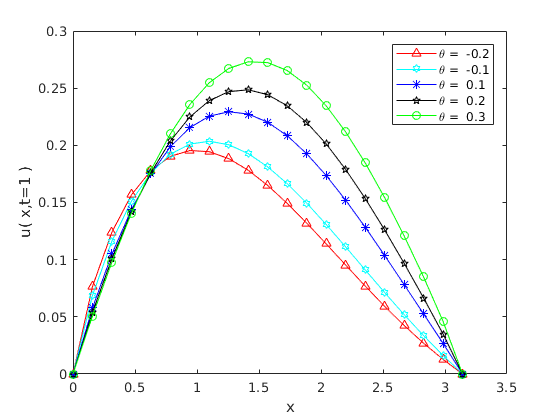
\includegraphics[scale=0.5]{theta.png}
	\caption{$\theta$取不同值,$\alpha=1.7$时,最后一步数值解的图像}
	\label{fig:pathdemo4}
\end{figure*}
图3.1、图3.2体现了带有不同倾斜度$\theta$的对流-扩散过程的不同。其中$\alpha=1.7$,$\theta=\pm 0.2,\pm 0.1,0.3$,a = 1.5,b = 1.0,$h=\pi/20$,$\tau=0.0001$。
\\
\\
\\
\\
\\
\\
\begin{figure*}[ht]	
	\centering
	\includegraphics[scale=0.6]{figure5.png}
	\caption{$\alpha$取不同值,$\theta=0.3$时最后一步的数值解u(x,t)}
	\label{fig:pathdemo4}
\end{figure*}

\begin{figure*}[ht]	
	\centering
	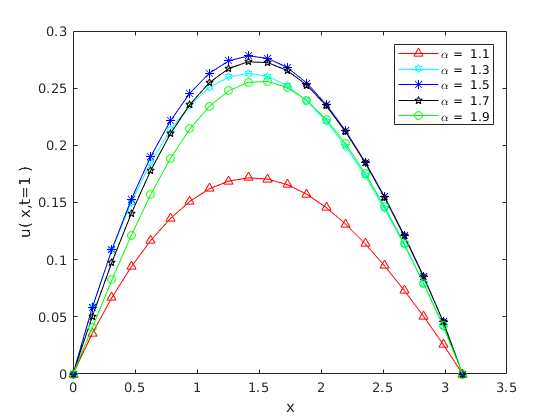
\includegraphics[scale=0.5]{alpha.png}
	\caption{$\alpha$取不同值,$\theta=0.3$时,最后一步数值解的图像}
	\label{fig:pathdemo4}
\end{figure*}

图3.3、图3.4给出了不同阶$\alpha$的对流-扩散过程的不同。其中$\alpha=1.1,1.3,1.5,1.7,1.9$,$\quad$$\theta=0.3$。
结合以上图像可知,$\alpha$一定时,函数的振幅随$\theta$的增大而增大,不同的是,$\theta$一定时,$\alpha$=1.5时振幅最大,并没有呈现出与变量$\alpha$正相关的规律。
\\
\\
\\
\\
\\
\\
\\
\\
\begin{figure}[h]
	\begin{minipage}[t]{0.4\linewidth}%并排放两张图片,每张占行的0.4,下同 
		\centering     %插入的图片居中表示
		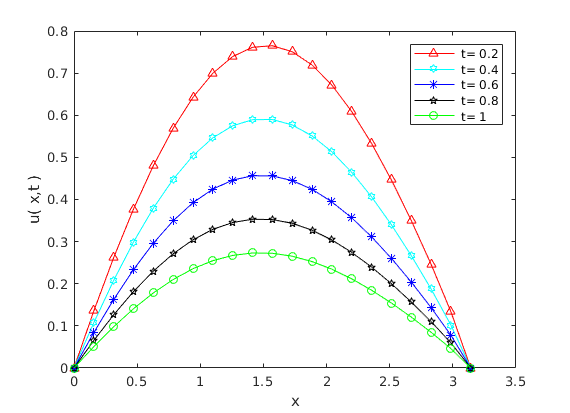
\includegraphics[width=1.2\textwidth]{t1.png}
		\caption{$t$取不同值时,最后一步数值解的图像}%图片的名称
		\label{fig:liuchengtu1}%标签,用作
	\end{minipage} 
	\hfill
	\begin{minipage}[t]{0.4\linewidth}
		\centering
		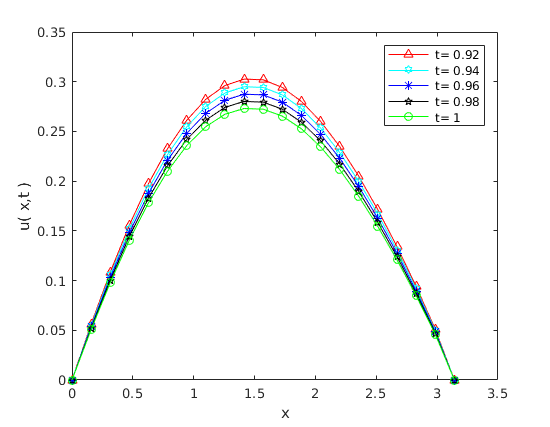
\includegraphics[width=1.2\textwidth]{t2.png}
		\caption{细化t剖分,$t$取不同值时,最后一步数值解的图像}%图片的名称
		\label{fig:liuchengtu2}
	\end{minipage}
\end{figure}

图3.5、图3.6描绘的是方程表示的对流-扩散过程。由图3.5可知,随着t的增大,u(x,t)的振幅逐渐减小,且趋于平缓,于是我们细化t的剖分,令$t=0.92、0.94、0.96、0.98、1.0$,结果如图3.6所示,u(x,t)振幅越来越小,且函数图像逼近$u(x,t=1.0)$,所以u(x,t)关于t是收敛的。

\subsubsection{稳定性分析}
我们给初值条件sin(x)加入一个微小干扰,即令$o(h)=\pi/20$,考虑初值条件为sin(x+o(h))时的数值解,得到的图象如下:
\begin{figure}[h]
	\begin{minipage}[t]{0.4\linewidth}%并排放两张图片,每张占行的0.4,下同 
		\centering     %插入的图片居中表示
		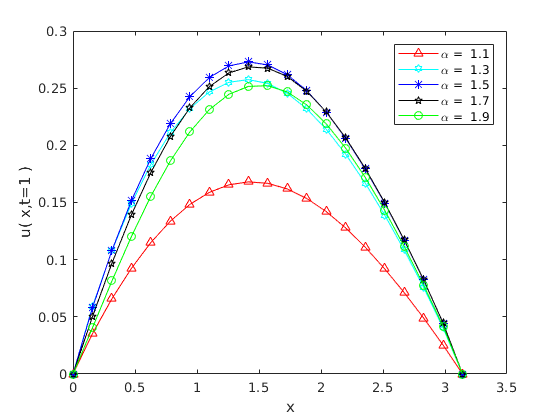
\includegraphics[width=1.2\textwidth]{alpha+o.png}
		\caption{x+o(h)后,$\alpha$取不同值,$\theta=0.3$时,最后一步数值解的图像}%图片的名称
		\label{fig:liuchengtu1}%标签,用作
	\end{minipage} 
	\hfill
	\begin{minipage}[t]{0.4\linewidth}
		\centering
		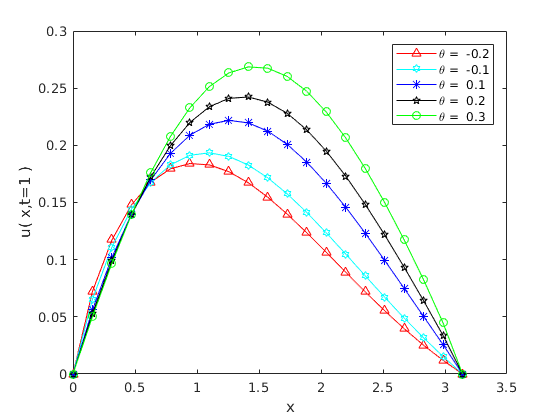
\includegraphics[width=1.2\textwidth]{theta+o.png}
		\caption{x+o(h)后,$\theta$取不同值,$\alpha=1.7$时,最后一步数值解的图像}%图片的名称
		\label{fig:liuchengtu2}
	\end{minipage}
\end{figure}
\\
\\
\\
\begin{figure}[h]
	\begin{minipage}[t]{0.4\linewidth}%并排放两张图片,每张占行的0.4,下同 
		\centering     %插入的图片居中表示
		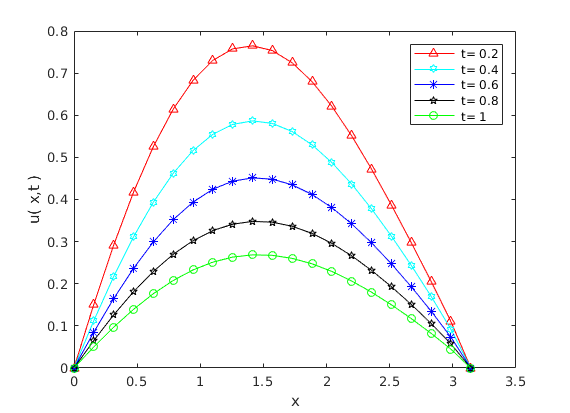
\includegraphics[width=1.2\textwidth]{t1+o.png}
		\caption{x+o(h)后,$t$取不同值时,最后一步数值解的图像}%图片的名称
		\label{fig:liuchengtu1}%标签,用作
	\end{minipage} 
	\hfill
	\begin{minipage}[t]{0.4\linewidth}
		\centering
		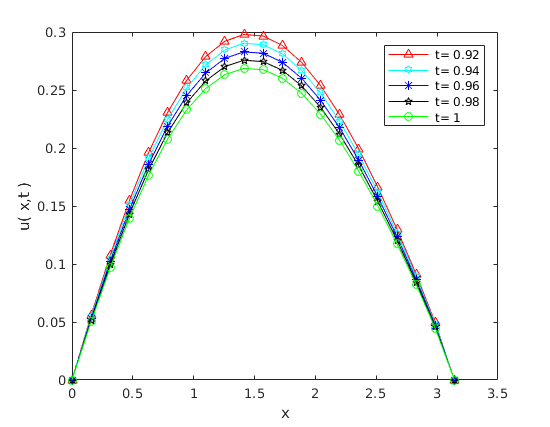
\includegraphics[width=1.2\textwidth]{t2+o.png}
		\caption{细化t剖分,$t$取不同值时,最后一步数值解的图像}%图片的名称
		\label{fig:liuchengtu2}
	\end{minipage}
\end{figure}

通过与初值条件为sin(x)时的图像比较,我们直观地看到其结果的变化是微小的,故我们认为该格式是稳定的。
